\documentclass[12pt, titlepage]{article}

\usepackage{fullpage}
\usepackage[round]{natbib}
\usepackage{multirow}
\usepackage{booktabs}
\usepackage{tabularx}
\usepackage{graphicx}
\usepackage{float}
\usepackage{hyperref}
\usepackage{longtable}
\hypersetup{
    colorlinks,
    citecolor=blue,
    filecolor=black,
    linkcolor=red,
    urlcolor=blue
}

%% Comments

\usepackage{color}

\newif\ifcomments\commentstrue %displays comments
%\newif\ifcomments\commentsfalse %so that comments do not display

\ifcomments
\newcommand{\authornote}[3]{\textcolor{#1}{[#3 ---#2]}}
\newcommand{\todo}[1]{\textcolor{red}{[TODO: #1]}}
\else
\newcommand{\authornote}[3]{}
\newcommand{\todo}[1]{}
\fi

\newcommand{\wss}[1]{\authornote{blue}{SS}{#1}} 
\newcommand{\plt}[1]{\authornote{magenta}{TPLT}{#1}} %For explanation of the template
\newcommand{\an}[1]{\authornote{cyan}{Author}{#1}}

%% Common Parts

\newcommand{\progname}{ProgName} % PUT YOUR PROGRAM NAME HERE
\newcommand{\authname}{Team \#, Team Name
\\ Student 1 name
\\ Student 2 name
\\ Student 3 name
\\ Student 4 name} % AUTHOR NAMES                  

\usepackage{hyperref}
    \hypersetup{colorlinks=true, linkcolor=blue, citecolor=blue, filecolor=blue,
                urlcolor=blue, unicode=false}
    \urlstyle{same}
                                


\newcounter{acnum}
\newcommand{\actheacnum}{AC\theacnum}
\newcommand{\acref}[1]{AC\ref{#1}}

\newcounter{ucnum}
\newcommand{\uctheucnum}{UC\theucnum}
\newcommand{\uref}[1]{UC\ref{#1}}

\newcounter{mnum}
\newcommand{\mthemnum}{M\themnum}
\newcommand{\mref}[1]{M\ref{#1}}

\begin{document}

\title{Module Guide for \progname{}} 
\author{\authname}
\date{\today}

\maketitle

\pagenumbering{roman}

\section{Revision History}

\begin{tabularx}{\textwidth}{p{3cm}p{2cm}X}
\toprule {\bf Date} & {\bf Version} & {\bf Notes}\\
\midrule
Date 1 & 1.0 & Notes\\
Date 2 & 1.1 & Notes\\
\bottomrule
\end{tabularx}

\newpage

\section{Reference Material}

This section records information for easy reference.

\subsection{Abbreviations and Acronyms}

\renewcommand{\arraystretch}{1.2}
\begin{tabular}{l l} 
  \toprule		
  \textbf{symbol} & \textbf{description}\\
  \midrule 
  AC & Anticipated Change\\
  DAG & Directed Acyclic Graph \\
  M & Module \\
  MG & Module Guide \\
  OS & Operating System \\
  R & Requirement\\
  SC & Scientific Computing \\
  SRS & Software Requirements Specification\\
  \progname & The name of the application being built\\
  UC & Unlikely Change \\
  CRUD & Create, Read, Update, Delete \\
  \wss{etc.} & \wss{...}\\
  \bottomrule
\end{tabular}\\

\newpage

\tableofcontents

\listoftables

\listoffigures

\newpage

\pagenumbering{arabic}

\section{Introduction}

Decomposing a system into modules is a commonly accepted approach to developing
software.  A module is a work assignment for a programmer or programming
team~\citep{ParnasEtAl1984}.  We advocate a decomposition
based on the principle of information hiding~\citep{Parnas1972a}.  This
principle supports design for change, because the ``secrets'' that each module
hides represent likely future changes.  Design for change is valuable in SC,
where modifications are frequent, especially during initial development as the
solution space is explored.  

Our design follows the rules layed out by \citet{ParnasEtAl1984}, as follows:
\begin{itemize}
\item System details that are likely to change independently should be the
  secrets of separate modules.
\item Each data structure is implemented in only one module.
\item Any other program that requires information stored in a module's data
  structures must obtain it by calling access programs belonging to that module.
\end{itemize}

After completing the first stage of the design, the Software Requirements
Specification (SRS), the Module Guide (MG) is developed~\citep{ParnasEtAl1984}. The MG
specifies the modular structure of the system and is intended to allow both
designers and maintainers to easily identify the parts of the software.  The
potential readers of this document are as follows:

\begin{itemize}
\item New project members: This document can be a guide for a new project member
  to easily understand the overall structure and quickly find the
  relevant modules they are searching for.
\item Maintainers: The hierarchical structure of the module guide improves the
  maintainers' understanding when they need to make changes to the system. It is
  important for a maintainer to update the relevant sections of the document
  after changes have been made.
\item Designers: Once the module guide has been written, it can be used to
  check for consistency, feasibility, and flexibility. Designers can verify the
  system in various ways, such as consistency among modules, feasibility of the
  decomposition, and flexibility of the design.
\end{itemize}

The rest of the document is organized as follows. Section
\ref{SecChange} lists the anticipated and unlikely changes of the software
requirements. Section \ref{SecMH} summarizes the module decomposition that
was constructed according to the likely changes. Section \ref{SecConnection}
specifies the connections between the software requirements and the
modules. Section \ref{SecMD} gives a detailed description of the
modules. Section \ref{SecTM} includes two traceability matrices. One checks
the completeness of the design against the requirements provided in the SRS. The
other shows the relation between anticipated changes and the modules. Section
\ref{SecUse} describes the use relation between modules.

\section{Anticipated and Unlikely Changes} \label{SecChange}

This section lists possible changes to the system. According to the likeliness
of the change, the possible changes are classified into two
categories. Anticipated changes are listed in Section \ref{SecAchange}, and
unlikely changes are listed in Section \ref{SecUchange}.

\subsection{Anticipated Changes} \label{SecAchange}

Anticipated changes are the source of the information that is to be hidden
inside the modules. Ideally, changing one of the anticipated changes will only
require changing the one module that hides the associated decision. The approach
adapted here is called design for
change.

\begin{description}
\item[\refstepcounter{acnum} \actheacnum \label{acHardware}:] The specific hardware on which the software is running.
\item[\refstepcounter{acnum} \actheacnum \label{acInput}:] The format of the initial receipt data.
\item[\refstepcounter{acnum} \actheacnum \label{acAPIReq}:] The structure of the data inputted to the server.
\item[\refstepcounter{acnum} \actheacnum \label{acAPIRes}:] The structure of the data returned from the server.
\item[\refstepcounter{acnum} \actheacnum \label{acFormat}:] The styling and formatting of UI components and user input.
\item[\refstepcounter{acnum} \actheacnum \label{acDB}:] The table structure of the databases.
\end{description}

\subsection{Unlikely Changes} \label{SecUchange}

The module design should be as general as possible. However, a general system is
more complex. Sometimes this complexity is not necessary. Fixing some design
decisions at the system architecture stage can simplify the software design. If
these decision should later need to be changed, then many parts of the design
will potentially need to be modified. Hence, it is not intended that these
decisions will be changed.

\begin{description}
\item[\refstepcounter{ucnum} \uctheucnum \label{ucIO}:] The user interface will be on a mobile device that has a camera for primary input.
\item[\refstepcounter{ucnum} \uctheucnum \label{ucIO}:] The server will run on NodeJS.
\item[\refstepcounter{ucnum} \uctheucnum \label{ucIO}:] The front end mobile app will be built on Flutter.
\item[\refstepcounter{ucnum} \uctheucnum \label{ucIO}:] The database will be PostgreSQL.

\end{description}

\section{Module Hierarchy} \label{SecMH}

This section provides an overview of the module design. Modules are summarized
in a hierarchy decomposed by secrets in Table \ref{TblMH}. The modules listed
below, which are leaves in the hierarchy tree, are the modules that will
actually be implemented.

\begin{description}
\item [\refstepcounter{mnum} \mthemnum \label{mHH}:] Hardware-Hiding Module
\item [\refstepcounter{mnum} \mthemnum \label{mRVision}:] Receipt Vision Module (OCR)
\item [\refstepcounter{mnum} \mthemnum \label{mReview}:] Receipt Extraction and Review
\item [\refstepcounter{mnum} \mthemnum \label{mLocation}:] Location Management Module
\item [\refstepcounter{mnum} \mthemnum \label{mAnalytics}:] User Analytics Module
\item [\refstepcounter{mnum} \mthemnum \label{mUsers}:] Users Module
\item [\refstepcounter{mnum} \mthemnum \label{mAuth}:] Authentication Module
\item [\refstepcounter{mnum} \mthemnum \label{mRec}:] Recommendation Engine
\item [\refstepcounter{mnum} \mthemnum \label{mClassification}:] Classification Engine
\item [\refstepcounter{mnum} \mthemnum \label{mDBDriver}:] Database Driver Module


\end{description}

Note that \ref{mHH} is a commonly used module and is already implemented by the operating system.
It will not be reimplemented.

\begin{table}[h!]
\centering
\begin{tabular}{p{0.3\textwidth} p{0.6\textwidth}}
\toprule
\textbf{Level 1} & \textbf{Level 2}\\
\midrule

{Hardware-Hiding Module} & ~ \\
\midrule

\multirow{7}{0.3\textwidth}{Behaviour-Hiding Module} & Receipt Vision Module (OCR)\\
& Receipt Extraction Module\\
& Location Management Module\\
& User Analytics Module\\
& Users Module\\
& Authentication Module\\
\midrule

\multirow{3}{0.3\textwidth}{Software Decision Module} & Recommendation Engine\\
& Classification Engine\\
& Database Driver Module\\
\bottomrule

\end{tabular}
\caption{Module Hierarchy}
\label{TblMH}
\end{table}

\section{Connection Between Requirements and Design} \label{SecConnection}

The design of the system is intended to satisfy the requirements developed in
the SRS. In this stage, the system is decomposed into modules. The connection
between requirements and modules is listed in Table~\ref{TblRT}.

\section{Module Decomposition} \label{SecMD}

Modules are decomposed according to the principle of ``information hiding''
proposed by \citet{ParnasEtAl1984}. The \emph{Secrets} field in a module
decomposition is a brief statement of the design decision hidden by the
module. The \emph{Services} field specifies \emph{what} the module will do
without documenting \emph{how} to do it. For each module, a suggestion for the
implementing software is given under the \emph{Implemented By} title. If the
entry is \emph{OS}, this means that the module is provided by the operating
system or by standard programming language libraries.  \emph{\progname{}} means the
module will be implemented by the \progname{} software.

Only the leaf modules in the hierarchy have to be implemented. If a dash
(\emph{--}) is shown, this means that the module is not a leaf and will not have
to be implemented.

\subsection{Hardware Hiding Modules (\mref{mHH})}

\begin{description}
\item[Secrets:]The data structure and algorithm used to implement the virtual
  hardware.
\item[Services:]Serves as a virtual hardware used by the rest of the
  system. This module provides the interface between the hardware and the
  software. So, the system can use it to display outputs or to accept inputs.
\item[Implemented By:] OS
\end{description}

\subsection{Behaviour-Hiding Module}

\begin{description}
\item[Secrets:]The contents of the required behaviours.
\item[Services:]Includes programs that provide externally visible behaviour of
  the system as specified in the software requirements specification (SRS)
  documents. This module serves as a communication layer between the
  hardware-hiding module and the software decision module. The programs in this
  module will need to change if there are changes in the SRS.
\item[Implemented By:] --
\end{description}

\subsubsection{Vision Module (\mref{mRVision})}

\begin{description}
\item[Secrets:] The dependencies and algorithms required to facilitate text recognition of receipts.
\item[Services:] Provides methods related to usage of the device camera and extraction of the text from captured
receipts.
\item[Implemented By:] Grocery Spending Tracker
\item[Type of Module:] Library
\end{description}

\subsubsection{Receipt Extraction Module (\mref{mExtraction})}

\begin{description}
\item[Secrets:] The algorithms required to extract relevant information from the scanned receipt text.
\item[Services:] Isolates necessary information from scanned receipt text, organizes it, and sends to other
modules.
\item[Implemented By:] Grocery Spending Tracker
\item[Type of Module:] Library
\end{description}

\subsubsection{Location Management Module (\mref{mLocation})}

\begin{description}
\item[Secrets:] The dependencies and algorithms for determining location-based relevance. 
\item[Services:] Determines relevance of information based on location data.
\item[Implemented By:] Grocery Spending Tracker
\item[Type of Module:] Library
\end{description}

\subsubsection{User Analytics Module (\mref{mAnalytics})}

\begin{description}
\item[Secrets:] The data structures and algorithms for compiling and computing user purchasing analytics. 
\item[Services:] Provide analytics and feedback on user purchasing behaviour, offering insight on recent and future purchasing.
\item[Implemented By:] Grocery Spending Tracker
\item[Type of Module:] Library
\end{description}

\subsubsection{Users Module (\mref{mUsers})}

\begin{description}
\item[Secrets:] The data structures that hold all user data such as goals and reciept data.
\item[Services:] Produce CRUD operations for operations related to users.
\item[Implemented By:] Grocery Spending Tracker
\item[Type of Module:] Library
\end{description}

\subsubsection{Authentication Module (\mref{mUsers})}

\begin{description}
\item[Secrets:] The data structures that hold all account data such as username, password, and email.
\item[Services:] Facilitates secure user login and authentication.
\item[Implemented By:] Grocery Spending Tracker
\item[Type of Module:] Library
\end{description}

\subsection{Software Decision Module}

\begin{description}
\item[Secrets:] The design decision based on mathematical theorems, physical
  facts, or programming considerations. The secrets of this module are
  \emph{not} described in the SRS.
\item[Services:] Includes data structure and algorithms used in the system that
  do not provide direct interaction with the user. 
  % Changes in these modules are more likely to be motivated by a desire to
  % improve performance than by externally imposed changes.
\item[Implemented By:] --
\end{description}

\subsubsection{Database Driver Module (\mref{mUsers})}

\begin{description}
\item[Secrets:] The data structures for representing the database schema and providing interface from the other modules.
\item[Services:] Facilitates communication between the database and the other modules.
\item[Implemented By:] Grocery Spending Tracker
\item[Type of Module:] Library
\end{description}

\section{Traceability Matrix} \label{SecTM}

This section shows two traceability matrices: between the modules and the
requirements and between the modules and the anticipated changes.

% the table should use mref, the requirements should be named, use something
% like fref
\begin{longtable}{p{0.2\textwidth} p{0.6\textwidth}}
\toprule
\textbf{Req.} & \textbf{Modules}\\
\midrule
FR1 & \mref{mAuth}\\
FR2 & \mref{mAuth}, \mref{mDBDriver}\\
FR3 & \mref{mRVision}\\
FR4 & \mref{mLocation}, \mref{mUsers}, \mref{mDBDriver}\\
FR5 & \mref{mUsers}, \mref{mDBDriver}\\
FR6 & \mref{mUsers}, \mref{mDBDriver}\\
FR7 & \mref{mClassification}, \mref{mDBDriver}\\
FR8 & \mref{mRec}, \mref{mDBDriver}\\
FR9 & \mref{mRec}, \mref{mDBDriver}\\
FR10 & \mref{mAnalytics}, \mref{mDBDriver}\\
FR11 & \mref{mReview}\\
FR12 & \mref{mClassification}, \mref{mDBDriver}\\
AR1 & \mref{mRVision}, \mref{mReview}, \mref{mLocation}, \mref{mAnalytics}, \mref{mUsers}, \mref{mAuth}, \mref{mRec}\\
AR2 & \mref{mRVision}, \mref{mReview}, \mref{mLocation}, \mref{mAnalytics}, \mref{mUsers}, \mref{mAuth}, \mref{mRec}\\
AR3 & \mref{mRVision}, \mref{mReview}, \mref{mLocation}, \mref{mAnalytics}, \mref{mUsers}, \mref{mAuth}, \mref{mRec}\\
SR1 & \mref{mRVision}, \mref{mReview}, \mref{mLocation}, \mref{mAnalytics}, \mref{mUsers}, \mref{mAuth}, \mref{mRec}\\
SR2 & \mref{mRVision}, \mref{mReview}, \mref{mLocation}, \mref{mAnalytics}, \mref{mUsers}, \mref{mAuth}, \mref{mRec}\\
SR3 & \mref{mRVision}, \mref{mReview}, \mref{mLocation}, \mref{mAnalytics}, \mref{mUsers}, \mref{mAuth}, \mref{mRec}\\
EUR1 & \mref{mRVision}, \mref{mReview}, \mref{mLocation}, \mref{mAnalytics}, \mref{mUsers}, \mref{mAuth}, \mref{mRec}\\
EUR2 & \mref{mRVision}, \mref{mReview}, \mref{mLocation}, \mref{mAnalytics}, \mref{mUsers}, \mref{mAuth}, \mref{mRec}\\
EUR3 & \mref{mRVision}, \mref{mReview}, \mref{mLocation}, \mref{mAnalytics}, \mref{mUsers}, \mref{mAuth}, \mref{mRec}\\
PIR1 & \mref{mRVision}, \mref{mReview}, \mref{mLocation}, \mref{mAnalytics}, \mref{mUsers}, \mref{mAuth}, \mref{mRec}\\
PIR2 & \mref{mRVision}, \mref{mReview}, \mref{mLocation}, \mref{mAnalytics}, \mref{mUsers}, \mref{mAuth}, \mref{mRec}\\
PIR3 & \mref{mUsers}\\
LR1 & \mref{mRVision}, \mref{mReview}, \mref{mLocation}, \mref{mAnalytics}, \mref{mUsers}, \mref{mAuth}, \mref{mRec}\\
LR2 & \mref{mRVision}, \mref{mReview}, \mref{mLocation}, \mref{mAnalytics}, \mref{mUsers}, \mref{mAuth}, \mref{mRec}\\
UPR1 & \mref{mRVision}, \mref{mReview}, \mref{mLocation}, \mref{mAnalytics}, \mref{mUsers}, \mref{mAuth}, \mref{mRec}\\
UPR2 & \mref{mRVision}, \mref{mReview}, \mref{mLocation}, \mref{mAnalytics}, \mref{mUsers}, \mref{mAuth}, \mref{mRec}\\
ACR1 & \mref{mRVision}, \mref{mReview}, \mref{mLocation}, \mref{mAnalytics}, \mref{mUsers}, \mref{mAuth}, \mref{mRec}\\
ACR2 & \mref{mRVision}, \mref{mReview}, \mref{mLocation}, \mref{mAnalytics}, \mref{mUsers}, \mref{mAuth}, \mref{mRec}\\
SLR1 & \mref{mRVision}, \mref{mReview}, \mref{mLocation}, \mref{mAnalytics}, \mref{mUsers}, \mref{mAuth}, \mref{mRec}, \mref{mClassification}, \mref{mDBDriver}\\
SLR2 & \mref{mRVision}, \mref{mReview}, \mref{mLocation}, \mref{mAnalytics}, \mref{mUsers}, \mref{mAuth}, \mref{mRec}\\
PAR1 & \mref{mRVision}, \mref{mReview}, \mref{mLocation},\mref{mAnalytics}, \mref{mUsers}, \mref{mAuth}\\
PAR2 & \mref{mAnalytics}\\
RFR1 & \mref{mRVision}, \mref{mReview}, \mref{mLocation},\mref{mAnalytics}, \mref{mUsers}, \mref{mAuth}\\
CR1 & \mref{mRVision}, \mref{mReview}, \mref{mLocation}, \mref{mAnalytics}, \mref{mUsers}, \mref{mAuth}, \mref{mRec}, \mref{mClassification}\\
EPER1 & \mref{mRVision}, \mref{mReview}, \mref{mLocation}, \mref{mAnalytics}, \mref{mUsers}, \mref{mAuth}, \mref{mRec}, \mref{mClassification}\\
EPER2 & \mref{mRVision}, \mref{mReview}, \mref{mLocation}, \mref{mAnalytics}, \mref{mUsers}, \mref{mAuth}, \mref{mRec}, \mref{mClassification}\\
EPER3 & \mref{mRVision}, \mref{mReview}, \mref{mLocation}, \mref{mAnalytics}, \mref{mUsers}, \mref{mAuth}, \mref{mRec}, \mref{mClassification}\\
WER1 & \mref{mRVision}\\
WER2 & \mref{mReview}, \mref{mLocation}, \mref{mAnalytics}, \mref{mUsers}, \mref{mAuth}, \mref{mRec}, \mref{mClassification}\\
IASR1 & \mref{mRVision}, \mref{mReview}, \mref{mLocation}, \mref{mAnalytics}, \mref{mUsers}, \mref{mAuth}, \mref{mRec}, \mref{mClassification}\\
IASR2 & \mref{mRVision}, \mref{mReview}, \mref{mLocation}, \mref{mAnalytics}, \mref{mUsers}, \mref{mAuth}, \mref{mRec}, \mref{mClassification}\\
SPR1 & \mref{mRVision}, \mref{mReview}, \mref{mLocation}, \mref{mAnalytics}, \mref{mUsers}, \mref{mAuth}, \mref{mRec}\\
SPR2 & \mref{mRVision}, \mref{mReview}, \mref{mLocation}, \mref{mAnalytics}, \mref{mUsers}, \mref{mAuth}, \mref{mRec}, \mref{mClassification}\\
APR1 & \mref{mRVision}, \mref{mReview}, \mref{mLocation}, \mref{mAnalytics}, \mref{mUsers}, \mref{mAuth}, \mref{mRec}, \mref{mClassification}\\
APR2 & \mref{mRVision}, \mref{mReview}, \mref{mLocation}, \mref{mAnalytics}, \mref{mUsers}, \mref{mAuth}, \mref{mRec}, \mref{mClassification}, \mref{mDBDriver}\\
ACR1 & \mref{mRVision}, \mref{mReview}, \mref{mLocation}, \mref{mAnalytics}, \mref{mUsers}, \mref{mAuth}, \mref{mRec}, \mref{mClassification}, \mref{mDBDriver}\\
INR1 & \mref{mRVision}, \mref{mReview}, \mref{mLocation}, \mref{mAnalytics}, \mref{mUsers}, \mref{mAuth}, \mref{mRec}, \mref{mClassification}, \mref{mDBDriver}\\
INR2 & \mref{mRVision}, \mref{mReview}, \mref{mLocation}, \mref{mAnalytics}, \mref{mUsers}, \mref{mAuth}, \mref{mRec}, \mref{mClassification}, \mref{mDBDriver}\\
PRR1 & \mref{mRVision}, \mref{mReview}, \mref{mLocation}, \mref{mAnalytics}, \mref{mUsers}, \mref{mAuth}, \mref{mRec}, \mref{mClassification}, \mref{mDBDriver}\\
PRR2 & \mref{mRVision}, \mref{mReview}, \mref{mLocation}, \mref{mAnalytics}, \mref{mUsers}, \mref{mAuth}, \mref{mRec}, \mref{mClassification}, \mref{mDBDriver}\\
AUR1 & \mref{mRVision}, \mref{mReview}, \mref{mLocation}, \mref{mAnalytics}, \mref{mUsers}, \mref{mAuth}, \mref{mRec}, \mref{mClassification}, \mref{mDBDriver}\\
CUR1 & \mref{mRVision}, \mref{mReview}, \mref{mLocation}, \mref{mAnalytics}, \mref{mUsers}, \mref{mAuth}, \mref{mRec}, \mref{mClassification}, \mref{mDBDriver}\\
CUR2 & \mref{mRVision}, \mref{mReview}, \mref{mLocation}, \mref{mAnalytics}, \mref{mUsers}, \mref{mAuth}, \mref{mRec}, \mref{mClassification}, \mref{mDBDriver}\\
CUR3 & \mref{mRVision}, \mref{mReview}, \mref{mLocation}, \mref{mAnalytics}, \mref{mUsers}, \mref{mAuth}, \mref{mRec}, \mref{mClassification}, \mref{mDBDriver}\\
LR1 & \mref{mRVision}, \mref{mReview}, \mref{mLocation}, \mref{mAnalytics}, \mref{mUsers}, \mref{mAuth}, \mref{mRec}, \mref{mClassification}, \mref{mDBDriver}\\
LR2 & \mref{mRVision}, \mref{mReview}, \mref{mLocation}, \mref{mAnalytics}, \mref{mUsers}, \mref{mAuth}, \mref{mRec}, \mref{mClassification}, \mref{mDBDriver}\\
\bottomrule
\caption{Trace Between Requirements and Modules}
\label{TblRT}
\end{longtable}

\begin{table}[H]
\centering
\begin{tabular}{p{0.2\textwidth} p{0.6\textwidth}}
\toprule
\textbf{AC} & \textbf{Modules}\\
\midrule
\acref{acHardware} & \mref{mHH}\\
\acref{acInput} & \mref{mRVision}, \mref{mReview}\\
\acref{acAPIReq} & \mref{mReview}, \mref{mLocation}, \mref{mUsers}, \mref{mAuth}, \mref{mRec}, \mref{mClassification}\\
\acref{acAPIRes} & \mref{mAnalytics}, \mref{mLocation}, \mref{mUsers}, \mref{mAuth}, \mref{mRec}, \mref{mClassification}\\
\acref{acFormat} & \mref{mRVision}, \mref{mReview}, \mref{mLocation}, \mref{mAnalytics}, \mref{mUsers}, \mref{mAuth}, \mref{mRec}\\
\acref{acDB} & \mref{mDBDriver}\\
\bottomrule
\end{tabular}
\caption{Trace Between Anticipated Changes and Modules}
\label{TblACT}
\end{table}

\section{Use Hierarchy Between Modules} \label{SecUse}

In this section, the uses hierarchy between modules is
provided. \citet{Parnas1978} said of two programs A and B that A {\em uses} B if
correct execution of B may be necessary for A to complete the task described in
its specification. That is, A {\em uses} B if there exist situations in which
the correct functioning of A depends upon the availability of a correct
implementation of B.  Figure \ref{FigUH} illustrates the use relation between
the modules. It can be seen that the graph is a directed acyclic graph
(DAG). Each level of the hierarchy offers a testable and usable subset of the
system, and modules in the higher level of the hierarchy are essentially simpler
because they use modules from the lower levels.

\begin{figure}[H]
\centering
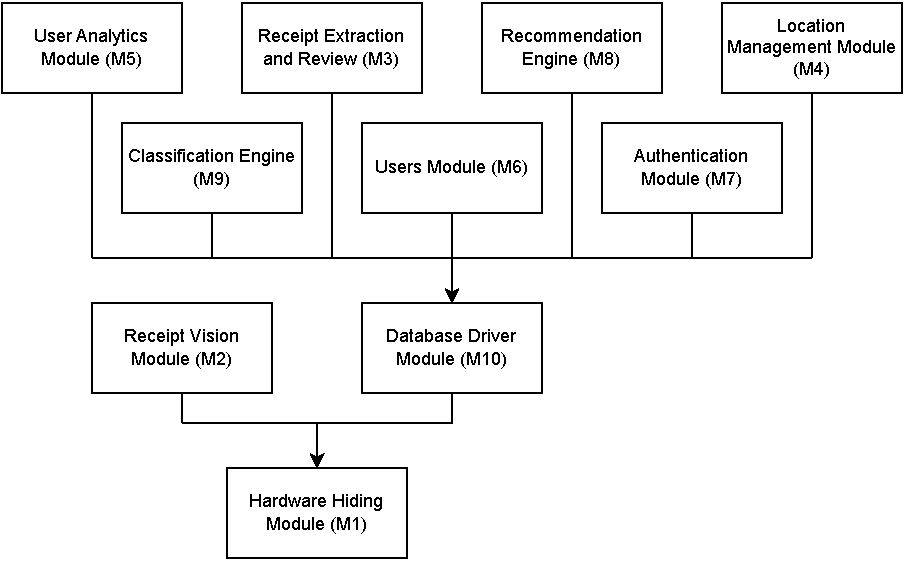
\includegraphics[width=0.8\textwidth]{./res/modulehierarchy.pdf}
\caption{Use hierarchy among modules}
\label{FigUH}
\end{figure}

\section{Timeline}

\subsection{Module Development Timeline}

Development of modules started in December 2023 and will continue into January 2024. Table \ref{ModuleDevelopmentTimeline}
shows the different modules being developed as well as the developer(s) who will be taking the lead
on it. This means they will be responsible for the primary planning and coding of the module. Developers not listed
on a module will still take part in development but on a more adhoc basis or as assistance is needed.
The timeline is also shown graphically in Figure \ref{FigureModuleDevelopmentTimeline}.

\begin{table}[H]
  \caption{Module Development Timeline}\label{ModuleDevelopmentTimeline}
  \begin{tabular}{|p{0.32\textwidth}|p{0.4\textwidth}|p{0.23\textwidth}|}
    \hline
    \textbf{Module Name} & \textbf{Development Start/End Date} & \textbf{Developer(s)} \\
    \hline
    Database Driver Module & Dec. 3 2023 \textemdash{} Jan. 31, 2024 & Jason Nam, Sawyer Tang, Ryan Yeh, Allan Fang \\
    \hline
    Recommendation Engine & Dec. 3 2023 \textemdash{} Jan. 31, 2024 & Jason Nam \\
    \hline
    Classification Engine & Dec. 3, 2023 \textemdash{} Jan 31, 2024 & Jason Nam\\
    \hline
    Receipt Vision Module & Dec. 3 2023 \textemdash{} Dec. 23, 2023 & Ryan Yeh \\
    \hline
    Receipt Extraction Module & Dec. 23, 2023 \textemdash{} Jan. 20, 2024 & Ryan Yeh \\
    \hline
    User Analytics Module & Dec. 23, 2023 \textemdash{} Jan. 20, 2024 & Allan Fang \\
    \hline
    Location Management Module & Jan. 1, 2024 \textemdash{} Jan. 20, 2024 & Allan Fang \\
    \hline
    Authentication Module & Jan. 1, 2024 \textemdash{} Jan. 31, 2024 & Sawyer Tang \\
    \hline
    Users Module & Jan. 1, 2024 \textemdash{} Jan. 31, 2024 & Sawyer Tang \\
    \hline
  \end{tabular}
\end{table}

\begin{figure}[H]
  \centering
  \caption{Graphical Module Development Timeline}\label{FigureModuleDevelopmentTimeline}
  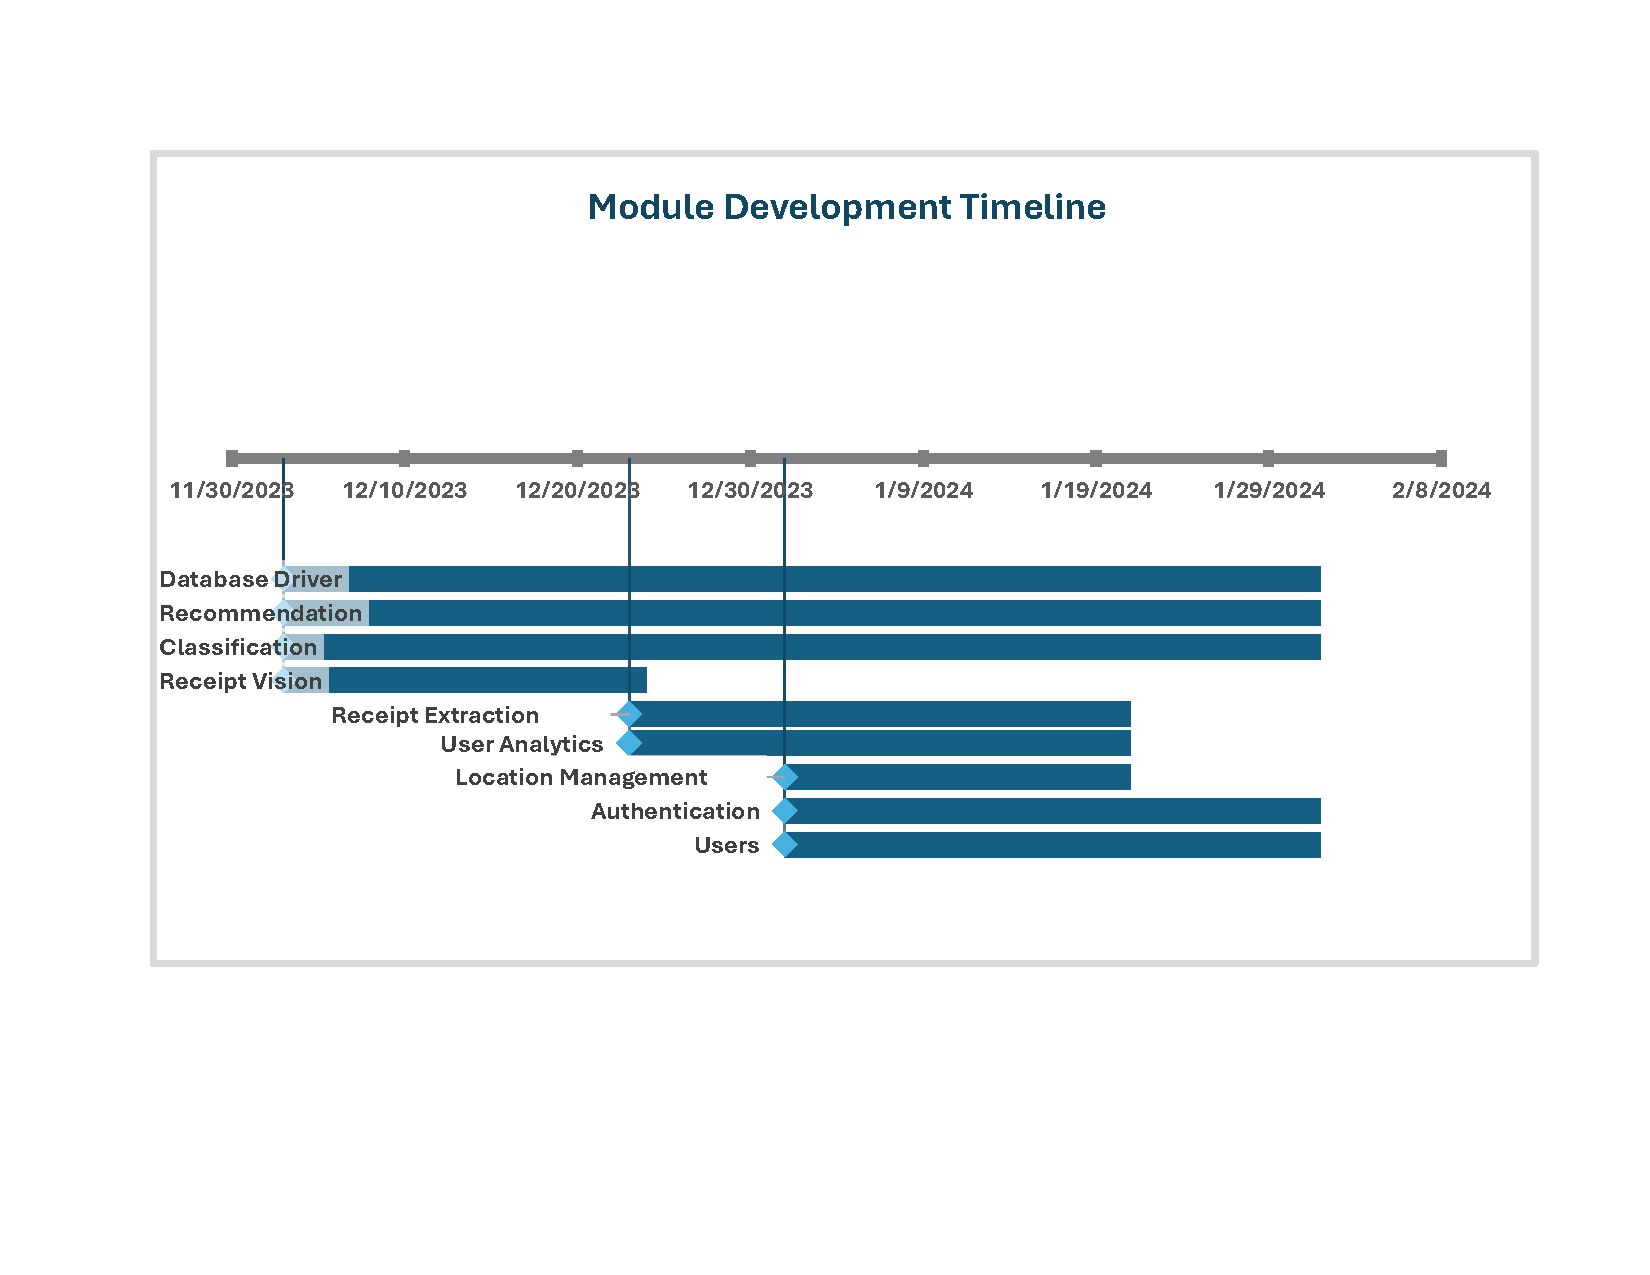
\includegraphics[width=0.8\textwidth]{./res/ModuleDevTimeline.pdf}
\end{figure}

\subsection{Module Testing Timeline}

Testing of modules also takes place during the development window set in the previous section. In general,
testing will involve basic manual testing of the application features to build confidence for the
Revision 0 Demo. For modules whose development end date is prior to January 31, testing will take place
during the following week. For the other modules, testing will largely take place concurrently with development
and small unit tests will be performed as the modules are created. The developers in charge of testing will
generally involve the main developer as written in Table \ref{ModuleDevelopmentTimeline} in addition to another developer
to help test the module with a fresher perspective. The details can be found in Table \ref{ModuleTestingTimeline} and graphically shown
in Figure \ref{FigureModuleTestingTimeline}.

\begin{table}[H]
  \caption{Module Testing Timeline}\label{ModuleTestingTimeline}
  \begin{tabular}{|p{0.32\textwidth}|p{0.4\textwidth}|p{0.23\textwidth}|}
    \hline
    \textbf{Module Name} & \textbf{Testing Start/End Date} & \textbf{Developer(s)} \\
    \hline
    Database Driver Module & Dec. 3 2023 \textemdash{} Jan. 31, 2024 & Jason Nam, Sawyer Tang, Ryan Yeh, Allan Fang \\
    \hline
    Recommendation Engine & Dec. 3 2023 \textemdash{} Jan. 31, 2024 & Jason Nam, Sawyer Tang \\
    \hline
    Classification Engine & Dec. 3, 2023 \textemdash{} Jan 31, 2024 & Jason Nam, Ryan Yeh\\
    \hline
    Receipt Vision Module & Dec. 23, 2023 \textemdash{} Dec 30, 2023 & Ryan Yeh, Allan Fang \\
    \hline
    Receipt Extraction Module & Jan. 20, 2023 \textemdash{} Jan. 27, 2024 & Ryan Yeh, Jason Nam \\
    \hline
    User Analytics Module & Jan. 20, 2024 \textemdash{} Jan. 27, 2024 & Allan Fang, Sawyer Tang \\
    \hline
    Location Management Module & Jan. 20, 2024 \textemdash{} Jan. 27, 2024 & Allan Fang, Ryan Yeh \\
    \hline
    Authentication Module & Jan. 1, 2024 \textemdash{} Jan. 31, 2024 & Sawyer Tang, Allan Fang \\
    \hline
    Users Module & Jan. 1, 2024 \textemdash{} Jan. 31, 2024 & Sawyer Tang, Jason Nam \\
    \hline
  \end{tabular}
\end{table}

\begin{figure}[H]
  \centering
  \caption{Graphical Module Testing Timeline}\label{FigureModuleTestingTimeline}
  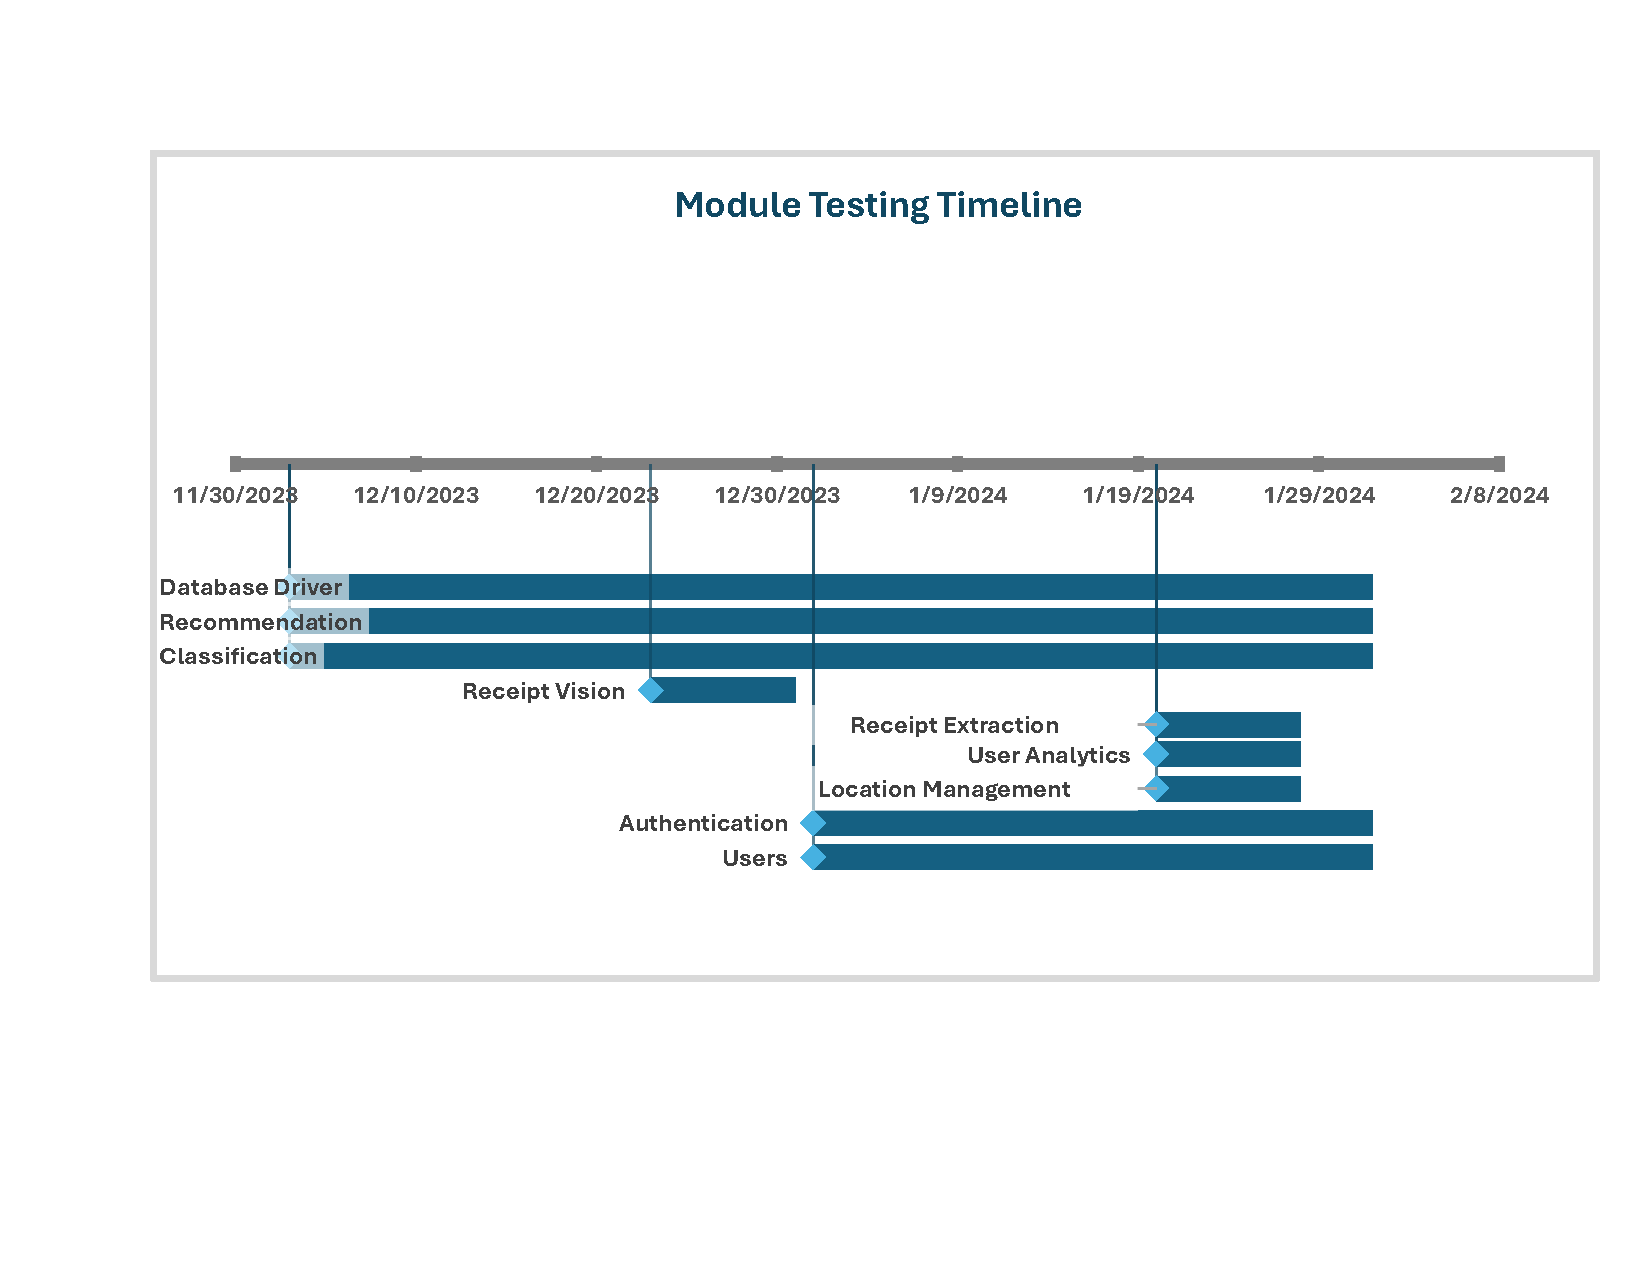
\includegraphics[width=0.8\textwidth]{./res/ModuleTestTimeline.pdf}
\end{figure}

%\section*{References}

\bibliographystyle {plainnat}
\bibliography{../../../refs/References}

\newpage{}

\end{document}